\section{Special Graph Classes}

\subsection{Eulerian Graphs}

\begin{definition}
An \dt{Eulerian trail}, which can be open or closed, is a trail where no edge is repeated and every edge is used. In a closed trail or \dt{Eulerian tour}, start = end.
\end{definition}

\begin{definition}
A graph is called \dt{Eulerian} if there is an Eulerian tour.
\end{definition}

\textbf{Theorem.}
Let $G=(V,E)$ be an undirected, connected multigraph. Then
\[
  G\text{ is Eulerian} \iff \forall x\in V: d(x)\text{ even}.
\]

There is an \emph{open} Eulerian trail $\iff$ exactly two vertices have odd degree.

\textbf{Proof.}
% "<==" direction
Proof by induction on $\alpha_1(G) =: m$.

$m = 0$: Trivial, only one vertex.

$m ≥ 1$: construct a tour $W$. You can always find a tour because degrees are even, thus every time you enter a vertex you can certainly find an edge where you can leave it.

Two cases:
a) $W$ is an Eulerian tour
b) $W$ is not an Eulerian tour

Then remove $W$, resulting in a graph $G'$ with connected components $G'_1$,~\ldots Then
\[
    \forall x\in V(G'_{i}): d_{G'}(x)\text{ is still even}
\]

Since all $G'_{i}$ are smaller than $G$, we can apply the induction hypothesis. This means $G'_{i}$ must be Eulerian (with Eulerian tours $W_{i}$).

$\forall i: W_i$ and $W$ have common vertex. Thus you can construct an Eulerian tour for the whole graph.

% Slides: Eulerian tour (started at 09:57... :)

% "==>" direction

Walk on an Eulerian tour.

\subsection{Hamiltonian Graphs}


\begin{definition}
In a \dt{Hamiltonian cycle}, each vertex is visited exactly once (except start/end).
$\text{$G$ is \dt{Hamiltonian}} \iff \exists\;\text{Hamiltonian cycle}.$
\end{definition}

Finding a Hamiltonian cycle in a graph is an NP-complete problem.

\begin{definition}
Let $G=(V,E)$ be a graph.
\[
%\forall v,w\in V :  \rightarrow\text{add $vw$ to $E$}\leadsto \tilde E
\tilde E = E\cup \{vw \mid v,w\in V,\; d(v)+d(w) ≥ |V|\}
\]
Then $[G] = (V,\tilde E)$ is called the \dt{closure} of $G$.
\end{definition}

\Theorem.  $G\text{ Hamiltonian} \iff [G]\text{ Hamiltonian}.$

\ProofForward.
Trivial.

\ProofBackward.
Choose
\begin{gather*}
  v,w\in V: vw \not\in E(G),\;d(v)+d(w) ≥ |V| \\
  H=(V,E\cup \{vw\})
\end{gather*}
Assume $H$ is Hamiltonian and $G$ is not.
This means that $\exists\;\text{Hamiltonian cycle in $H$}$ and it must contain $vw$.
In $H$ containing $vw$, say
\[ v=x_1,x_2,x_3,\ldots,x_n=w,x_1 \qquad(n=|V|)\]
Let
\begin{align*}
    X &=\{x_i \mid x_{i-1}\in \Gamma_G(w), 3 ≤ i ≤ n-1 \}\quad\text{and} \\
    Y &=\{x_i \mid x_i\in \Gamma_G(v), 3 ≤ i ≤ n-1 \}.
\end{align*}

\path{v, x_2, x_3, \ldots, x_{n-1}, w} is a path in $G$.

$v \not\in \Gamma_G(w) \implies |X| = d_G(w) - 1$
because exactly one neighbour is excluded, all the others are counted. $x_1= v$ is not a neighbour by our assumption.

$x_2, x_3, \ldots x_{n-2}$ there is one neighbour $x_{n-1}$ of $w$ which is not counted.

Analogously,
$|Y| = d_G(v) - 1$.

Thus $|X| + |Y| \geq n-2$.

Therefore, $\exists\,i: 3 ≤ i ≤ n-1$ such that
$x_{i-1}\in \Gamma_G(w), x_i\in\Gamma_G(v)$, because we iterate over $n-3$ values.

$\implies \path{v=x_1, x_i, x_{i+1}, \ldots, x_{n-1}, w=x_n, x_{i-1}, x_{i-2}, \ldots, x_2, v=x_1}$

But this is a Hamiltonian cycle in $G$ (contradiction).

If $H$ is not Hamiltonian, you could add other edges, but by the same argument, this will not lead to a Hamiltonian graph.

\textbf{Corollary 1.}
Let $G=(V,E), |V| ≥ 3$, such that
\[
    \forall v,w\in V: vw\not\in E\implies d(v) + d(w) \geq |V|.
\]
Then $G$ is Hamiltonian.

\textbf{Corollary 2.}
If
$\forall v \in V : d(v) \geq \frac{n}{2}$,
then $G$ is Hamiltonian.

The generalization of this problem, where you want to find an optimal Hamiltonian cycle in a weighted graph, is known as the \emph{Traveling Salesman Problem}.


\subsection{Planar Graphs}

\begin{definition}
A graph $G$ is \dt{planar} if there is an isomorphic graph $H$ embedded in the plane ($= \mathbb{R}^2$) such that no two edges intersect.
\end{definition}

\textbf{Examples for planar and non-planar Graphs}
\begin{figure}[htb]
  \centering
  \subfloat[$K_3$, planar]{
    \begin{tikzpicture}
      \fullyConnectedGraph{90,-30,180+30}{1cm}
    \end{tikzpicture}
  }
  \subfloat[$K_4$, planar]{
    \begin{tikzpicture}
      \fullyConnectedGraph{90-45, 90+45, -90-45, -90+45}{1cm}
    \end{tikzpicture}
  }
  \subfloat[$K_4$, planar, alternative]{
    \begin{tikzpicture}
      \fullyConnectedGraph{90,-30,180+30}{1cm}
      \node (n0) at (0,0) {};
      \fill (n0) circle(2pt);
      \foreach \i in {1,...,\the\value{nodecount}} {
	\path (n0) edge (n\i);
      };
    \end{tikzpicture}
  }
  \subfloat[$K_5$, nonplanar]{
    \begin{tikzpicture}
      \fullyConnectedGraph{90, 30, 180-30, -90-45, -90+45}{1.25cm}
    \end{tikzpicture}
  }
  \subfloat[$K_{3,3}$, nonplanar, bipartite]{
    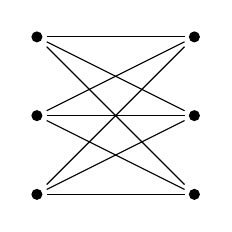
\begin{tikzpicture} % pipartite graph K_{3,3}
      \foreach \i in {1,...,3} {
	\node (n1\i) at (0,\i) {};
	\node (n2\i) at (2,\i) {};
	\fill (n1\i) circle(2pt);
	\fill (n2\i) circle(2pt);
      };
      \foreach \i in {1,...,3}
      {
	\foreach \j in {1,...,3}
	{
	  \path (n1\i) edge (n2\j);
	};
      };
    \end{tikzpicture}
  }
  \caption{Examples for (non-)planar Graphs}
\end{figure}


% triangle (planar)
% square with diagonals (planar) ≅ square with second diagonal non-intersecting
% K_5 (non-planar)
% bipartite graph K_{3,3} (non-planar)

$K_5$ is the smallest non-planar complete graph, $K_{3,3}$ is the smallest non-planar complete bipartite graph.

\begin{definition}
The edges of the graph (which have to be \emph{Jordan curves}) divide the plane into regions. These are the \dt{faces} of the planar graph.
\end{definition}

% Faces of K_4 - Inner: I, II, III, Outer: IV
\begin{figure}[htb] % K4 with the 4 faces labeled
  \centering
  \begin{tikzpicture}
    \fullyConnectedGraph{90,-30,180+30}{2cm}
    \node (n0) at (0,0) {};
    \fill (n0) circle(2pt);
    \foreach \i in {1,...,\the\value{nodecount}} {
      \path (n0) edge (n\i);
    };
    \node at (90+45:0.5cm) {I};
    \node at (45:0.5cm) {II};
    \node at (-90:0.5cm) {III};
    \node at (45:1.5cm) {IV};
  \end{tikzpicture}
  \caption{Faces of $K_4$}
\end{figure}




In the $K_4$, we get
\begin{align*}
    \alpha_0 &= 4 \\
    \alpha_1 &= 6 \\
    \alpha_2 &= 4\quad\text{number of faces}
\end{align*}

\begin{definition}
$H$ is a \dt{subdivision} of $G$ if $H$ is obtained by replacing every edge of $G$ by a path.
\end{definition}
% graph with 4 v and its graph with pathes

\begin{figure}[htb] % K4 and its subdivision
  \centering
  \subfloat[Graph $G$] {
    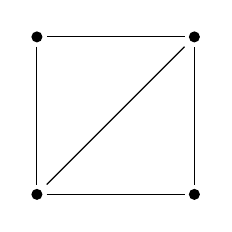
\begin{tikzpicture}
      \node (n1) at (0,0) {};
      \node (n2) at (2,0) {};
      \node (n3) at (2,2) {};
      \node (n4) at (0,2) {};
      \foreach \i in {1,...,4} {
	\fill (n\i) circle(2pt);
      };
      \foreach \i/\j in {1/2, 2/3, 3/4, 4/1, 1/3} {
	\path (n\i) edge (n\j);
      };
    \end{tikzpicture}
  }
  \subfloat[subdivision $H$ of $G$] {
    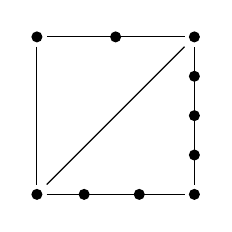
\begin{tikzpicture}
      \node (n1) at (0,0) {};
      \node (n2) at (2,0) {};
      \node (n3) at (2,2) {};
      \node (n4) at (0,2) {};
      \node (n5) at (0.6,0) {};
      \node (n6) at (1.3,0) {};
      \node (n7) at (2,.5) {};
      \node (n8) at (2,1.0) {};
      \node (n9) at (2,1.5) {};
      \node (n10) at (1,2) {};
      \foreach \i in {1,...,10} {
	\fill (n\i) circle(2pt);
      };
      \foreach \i/\j in {1/2, 2/3, 3/4, 4/1, 1/3} {
	\path (n\i) edge (n\j);
      };
    \end{tikzpicture}
  }
  \caption{Graph $G$ and one possible subdivision of $G$ named $H$}
\end{figure}




% Kuratovski's theorem?
\Theorem.
\[
    G\text{ planar} \iff \nexists\;\text{subgraph which is a subdivision of $K_5$ or of $K_{3,3}$.}
\]

\ProofBackward. Trivial if $K_5$ and $K_{3,3}$ non-planar.

\ProofForward. Too hard.

\textbf{Remark (Euler's polyhedron formula).}
\[
    G\text{ connected and planar} \implies
    \underbrace{\alpha_0 - \alpha_1 + \alpha_2}_
        {\text{Euler characteristic}}
    = 2.
\]

% figure of a polyhedron of a dice

\begin{figure}[htb] % polyhedron of a dice
  \centering
    \begin{tikzpicture}
      \drawGraph{1/1, 2/1, 2/2, 1/2, %
                 0/0, 3/0, 3/3, 0/3}%
		{1/2, 2/3, 3/4, 4/1, %
                 5/6, 6/7, 7/8, 8/5, %
	         1/5, 2/6, 3/7, 4/8}
    \end{tikzpicture}
  \caption{Polyhedron of a dice}
\end{figure}





\Proof.
Induction on $\alpha_2$.

Start with $\alpha_2=1$: $G$ is a tree. Then
\[
    \alpha_0-\alpha_1+1 = \alpha_0 - (\alpha_0 + 1) + 1 = 2.
\]

$\alpha_2 = k : k\rightarrow k+1: $
\[
    \text{$G$ has at least $k+1 \geq 2$ faces} \implies
    \exists\;\text{edge separating two faces}
\]
If we remove this edge, we get $G'$.
\begin{align*}
    \alpha_2(G') = k
    \implies &\alpha_0(G') - \alpha_1(G') + \alpha_2(G') = 2
    \implies &\alpha_0(G) - \alpha_1(G) + \alpha_2(G) = 2
\end{align*}

\Lemma.
If $G$ is planar, simple, no cycles of length $3$ (together, this also means no cycles of length $≤ 3$), connected, then
\[
    \alpha_1(G) ≤ 2\alpha_0(G) - 4.
\]

\Proof.
Let $f_j$ be the number of faces with a boundary of length $j$.
Then $f_3 = 0$.
\begin{align*}
\sum_{j≥4} f_j &= \alpha_2 \\
\sum_{j≥4} j f_j &≤ 2\alpha_1
    &&\text{ because each edge is counted at most twice.} \\
4 \sum_{j≥4} f_j ≤ 2\alpha_1
\end{align*}

%\TODO{figure 4 vertices, 3 faces}

\begin{align*}
    \alpha_0 - \alpha_1 + \alpha_2 &≥ 2 \\
    2\alpha_0 - 2\alpha_1 +
    \underbrace{2\alpha_2}_{≤ \alpha_1} &= 4 \\
    4 &≤ 2\alpha_0 - \alpha_1 \\
    \alpha_1 &≤ 2\alpha_0 - 4
\end{align*}

\Remark. In a graph with $k$ components, the Euler characteristic becomes
$\implies \alpha_0 - \alpha_1 + \alpha_2 = 1+k$

\textbf{Corollary.}
$K_{3,3}$ is not planar: Assume it is planar.
$\alpha_0 = 6, \alpha_1 = 9$. As a bipartite graph, it cannot have cycles of length 3: $f_3 = 0$. Therefore, we must have
\[
    \alpha_1 ≤ 2\alpha_0 - 4 \\
    9 ≤ 8
\]
Contradiction! Since $K_{3,3}$ satisfies all other requirements of the lemma, but the inequality does not hold, it cannot be planar.

\begin{definition}
Let $G=(V,E)$ be a planar graph and $F$ the set of faces.
Then $G^* = (V^*, E^*)$ is the \dt{dual} of $G$ with
\begin{align*}
&V^* = F. \\
&F_1F_2 \in E^* &&\text{if their boundaries have a common edge.}
\end{align*}
\end{definition}

% WRONG: \Remark. In general, $G^*$ is a multigraph.
\Remark. $G^*$ is not unique.
% WRONG: \Remark. $\forall v : d(v) ≠ 1 \implies |E| = |E^*|$

%%% corrections from 2013-10-24

\Remark.

\begin{compactenum}
  \item $|E| = |E^*|$
  \item In general $|G^*|$ is a multigraph
  \item $G_1, G_2$ are duals of $G \Rightarrow G_1 \cong G_2$
\end{compactenum}

$A \subseteq E$
$A$ cycle in $G \iff A^*$ minimal cut

If G is not necessarily planar: define $G^*$ by (*).
This Graph is unique, if it exists.

\textbf{Theorem (Witness Theorem).} \\
If G is not necessarily planar: define $G^{**}$ by (*)
\begin{compactitem}
  \item $G$ planar $\Rightarrow G^{**} \cong G^*$
  \item $G$ non planar $∄ G^{**}$
\end{compactitem}
% end of last weeks-corrections

\subsection{Bipartite Graphs and Matchings}

\begin{definition}
A simple, undirected graph $G=(V,E)$ is called \dt{bipartite}
iff
\begin{align*}
    V = V_1\cup V_2, V_1\cap V_2 = \varnothing \\
    vw\in E\implies v\in V_1, w\in V_2
\end{align*}
\end{definition}

$K_{n,m}$ is the complete bipartite graph.

\begin{definition}
$M\subseteq E$ is called a \dt{matching} if
\[
    \forall e,f\in M: e,f\text{ have no vertex in common.}
\]
\end{definition}
\begin{definition}
In a \dt{perfect matching},
\[
    \forall v\in V: v\text{ incident to some }e\in M.
\]
\end{definition}

\begin{figure}[htb] % perfect matching
  \centering
    \begin{tikzpicture}
      \drawGraph{0/0, 0/1, 0/2, 1/0, 1/1, 1/2}%
                {1/2, 2/3, 1/6, 1/4, 3/5, 4/5, 5/6}
      \foreach \i/\j in {1/5, 2/4, 3/6} {
	\draw[red, very thick] (n\i) -- (n\j);
      };
    \end{tikzpicture}
  \caption{Graph with perfect matching in red}
\end{figure}




\textbf{Theorem (Hall's marriage theorem).}
$W, M$ (women, men) vertex set of a bipartite graph
($V=W\cup M$, $wm \in E \iff w\operatorname{F}m$). $W,M$ finite, nonempty, $W\cap M=\varnothing$.

Friendship relation $F\subseteq W\times M$.

Feasible marriage: complete matching $F_1\subseteq F$, i.e.
\[ \forall x\in W: \exists!\;y\in M\text{ s.t. }x\operatorname{F} y \]

Theorem: There is a feasible marriage iff
\[
    \forall W_0\subseteq W:\;
        \underbrace{
            |\{y\in M\mid \exists x\in W_0: x\operatorname{F} y\}|
        }_{\bigcup\limits_{w\in W_0} \Gamma(w)}
        ≥ |W_0|
\]

If you have a feasable marriage, every woman gets a partner.
The Set of friends is at least this large

\Proof.
Consider the network source $s$ $\rightarrow_{w=1}$ women $\rightarrow_{w=|W|+|M|+1}$ men $\rightarrow_{w=1}$ sink $t$.
Since all weights are integer, $\exists$ maximal flow with integer weight.

\begin{figure}[htb]
  \centering
  \begin{tikzpicture}
    \drawDirGraph{0/0, 2/1.5, 2/0.5, 2/-0.5, 2/-1.5, 4/1.5, 4/0.5, 4/-0.5, 4/-1.5, 6/0}%
      { 1/2, 1/3, 1/4, 1/5, %
        6/10, 7/10, 8/10, 9/10, %
        2/6, 3/9, 4/7, 5/8}
    \draw[rounded corners,dashed] (1-0.5, 1.6) rectangle (1+0.5, -1.6);
    \draw[rounded corners,dashed] (5-0.5, 1.6) rectangle (5+0.5, -1.6);
    \draw[rounded corners,dashed] (3-0.5, 1.6) rectangle (3+0.5, -1.6);
    \node at (n1)[left] {$s$};
    \node at (n10)[right] {$t$};
    \node at (1,1.5)[above] {$w=1$};
    \node at (5,1.5)[above] {$w=1$};
    \node at (3,-1.5)[below] {$w=|W| + |M| + 1$};
  \end{tikzpicture}
  \caption{feasable marriage, $\exists$ maximal flow with integer weights}
\end{figure}


We claim that $S=(\{s\}, V \setminus \{s\})$
is a minimal cut ($c(S) = |W|$).

Assume $\exists S': c(S') < c(s)$. Then $S'$ has no edge $wm$ with $w\in W, m\in M$.

\[
S' = (V_1,V_2) \hat{=}
    \{sw\mid w \in \widetilde{W} \subseteq W \} \cup
    \{mt | m \in \widetilde{M} \subset M \}
\]

\def\GammaPlus{\Gamma^{+}}

We claim that
\[
    w\in W\setminus\widetilde{W}, m\in\GammaPlus(w)
    \implies m\in\widetilde{M}.
\]
Assume this does not hold. Then
\path{s, w, m, t} does not contain an edge of $S'$ $\implies s, t\in V_1$. Contradiction!

This implies that
\[
    |\bigcup\limits_{w\in W\setminus\widetilde{W}} \GammaPlus(w)|
    ≤ |\widetilde{M}|.
\]
But
\[
    c(S') = |\widetilde{W}| + |\widetilde{M}| < c(S) = |W|.
\]
This implies that
\[
    |\widetilde{M}| < |W\setminus \widetilde{W}|.
\]
Contradiction! Therefore $S'$ can not be a minimal cut. $S$ is proven to be a minimal cut.

The theorem of Ford-Fulkerson says that with a minimal cut,
$\exists\;\text{flow }\phi: v(\phi) = c(S) = |W|$. This flow defines the feasible marriage relation.


\subsection{Graph Colorings}

\begin{definition}
$G=(V,E)$ simple, undirected graph.
A \dt{vertex coloring} is a mapping
\[
    c : V\mapsto C, C=\{c_1,\ldots,c_r\}
\].
A coloring is \dt{feasible} if $vw\in E\implies c(v)≠c(w)$.
\end{definition}

\Remark. Edge coloring $\bar{c}: E\mapsto C$, feasible if edges with a common vertex have different colors.

\[
  \bar{G} = (\bar V, \bar E), \bar V = E \quad
  e_1 e_2\in \bar E \iff e_1,e_2\text{ share common vertex}
\]

\Remark. Similar: Face colorings of a planar graph (think of a map of countries)

\begin{definition}
$G=(V,E)$ graph. The \dt{chromatic number} $\chi(G)$ is the minimal number of colors so that there is a feasible coloring.
\end{definition}

Examples:
\begin{align*}
  &\chi(K_n) = n \\
  &\chi(K_{n,m}) = 2 \\
  &\chi(T) = 2 \text{ if $T$ tree, } |V| ≥ 1
\end{align*}

\Theorem.
\[
\begin{array}{r@{\quad}r@{ }l}
\text{1.} &
    \chi(G) = 1&\iff E(G) = \varnothing. \\
\text{2.} &
    \chi(G) = 2
        &\iff E(G) ≠ \varnothing, G\text{ bipartite} \\
        &&\iff E(G) ≠ \varnothing, \text{all cycles have even length}
\end{array}
\]

\Theorem.
$G$ planar $\implies \chi(G) \leq 4$. Proof is very hard!

\Theorem.
$\chi(G) ≤ 1 + \max{d(v)}.$

\Proof. By induction on $\alpha_0(G)$.

\Theorem. $G$ planar$\implies \chi(G) ≤ 5$.

\def\dmin{\ensuremath{d_{\text{min}}}}
\Proof.
Claim: In a planar graph, there is at least one vertex having at most five neighbors:
$\dmin ≤ 5$.

Assume $\dmin ≥ 6$.
Then
\[
  2\alpha_1 = \sum_{x\in V} d(x) ≥ 6\alpha_0\quad
  \alpha_1 ≥ \alpha_0.
\]
\[
  2\alpha_1 ≥
  \sum_{\text{faces}} \text{number of boundary edges} ≥
  3\alpha_2 =
  3 (2 - \alpha_0 + \alpha_1)
\]
\[
  \alpha_1 ≤ 3\alpha_0 - 6
\]

But $\alpha_1 ≥ 3\alpha_0$! Contradiction.

Cases: \\
\begin{compactenum}
%Case 1:
  \item $\dmin \leq 4$. Pick $x_0$ so that $d(x_0) \leq 4$.
Take $G' = G \setminus \{x_0\}$. Assume $\chi(G')=5$. Then, since $x_0$ has at most $4$ neighbors, you can color $x_0$ with the remaining color. By induction, $\chi(G)=5$.

%Case 2:
  \item $d_{\text{min}}=5$.
We have a vertex $v$ with exactly 5 neighbors $\{a,b,c,d,e\}$.
$c(a) = 1, c(b) = 2,\ldots$.
\\
$G_a = \{x\in V\mid \exists 1--3--1--3--\ldots \text{path a} \leadsto x\}$.
Similar for $G_c$.
  \begin{compactenum}
%Case 2.1:
    \item If $G_a\cap G_c =\varnothing$, we can recolor $G_a$ by switching colors 1 and 3. Then we can color $v$ with $c(v) = 1$.

%Case 2.2:
    \item If $G_a\cap G_c ≠ \varnothing$, then $G_a = G_c$.
%Case 2.2.1:
    \begin{compactenum}
      \item If $G_b\cap G_d =\varnothing$, then recolor $G_b$ by switching 2 and 4, and $c(v) = 2$.
%Case 2.2.2:
      \item If $G_b\cap G_d ≠\varnothing$, then $G_b = G_d$. Contradiction! (planar graph - the paths $G_a=G_c$ and $G_b=G_d$ cannot cross each other)
    \end{compactenum}
  \end{compactenum}
\end{compactenum}

\subsection{Ramsey Theory}

\textbf{Example.} Every 2-edge coloring of $K_6$ has a monochromatic $K_3$.

\begin{figure}[htb]
  \centering
  \subfigure[$K_6$]{
    \begin{tikzpicture}
      \fullyConnectedGraph{90-30, 90+30, 0, 180, 270-30,270+30}{1cm}
    \end{tikzpicture}
  }
  \subfigure[$K_3$]{
    \begin{tikzpicture}
      \fullyConnectedGraph{90+30, 270-30,0}{1cm}
    \end{tikzpicture}
  }
  \caption{$K_6$ and one $K_3$}
\end{figure}
\FloatBarrier

\TODO{Proof (graphical).}

\begin{definition}
The Ramsey number $R(r,s)$ is the minimum $n$ such that
every red-blue coloring of $K_n$ contains either a red $K_r$ or a blue $K_s$.
\end{definition}

By our example, $R(3,3) ≤ 6$. We can even show that $R(3,3) = 6$.

\TODO{figure out a good caption for Figure $K_5$}
\begin{figure}[htb]
  \centering
  \begin{tikzpicture}
    \fullyConnectedGraph{90, 30, 180-30, -90-45, -90+45}{1.25cm}
  \end{tikzpicture}
  \caption{$K_5$}
\end{figure}

Lemma. $R(r,s) ≤ R(r-1, s) + R(r, s-1)$

Proof. $n = R(r-1, s) + R(r, s-1)$
Partition $K_n$. Take a vertex $v$. All neighbors connected by a red edge are in $M$; all neighbors connected by a blue edge are in $N$.

$n = |M|+|N|+1$. Thus
\[
  |M| ≥ R(r-1, s) \text{ or } |N| ≥ R(r, s-1).
\]

\begin{tabular}{ll}
  Case 1: & $\exists$ blue $K_s$ in $M$ or $\exists$ red $K_{r-1}$ in $M$. \\
  Case 2: & $\exists$ blue $K_{s-1}$ in $M$ or red $K_r$ in $N$.
\end{tabular}

We wanted to show that $\exists$ blue $K_s$ or $\exists$ red $K_r$.
In both cases, \emph{together with $v$}, we can always find a blue $K_s$ or a red $K_r$.

\textbf{Corollary.} $R(r,s) ≤ {r+s-2 \choose r-1} ≤ 2^{r+s-2}$

\Proof. $R(2,n) = R(n,2) = n ≤ {n \choose 1}$. From there, apply induction, Pascal's triangle, and the above lemma.

\begin{definition}
\begin{align*}
  R(n_1,n_2,\ldots,n_r) = \min \{ n \mid
    &\text{ all r-edge colorings of $K_n$
      (colors $c_1,\ldots,c_r$)} \\
    & \text{ have a $c_j$-colored $K_j$ for some j}\}
\end{align*}
\end{definition}
